\documentclass[output=paper,colorlinks,citecolor=brown]{langscibook}
\ChapterDOI{10.5281/zenodo.10641191}
\author{Alexandra Rehn\orcid{}\affiliation{University of Konstanz}}
%\ORCIDs{}

\title[Parallel inflection in Old High German and Alemannic]{A new perspective on parallel inflection with reference to Old High German and Alemannic}


\abstract{Stacked adjectives in earlier as well as modern German varieties show so-called parallel inflection. This means that all adjectives must bear an inflectional ending. Inflecting only the left or rightmost adjective or varying the type of inflection (weak/strong) leads to ungrammaticality. Zero-inflected adjectives are also possible, i.e.~zero-inflection is iterated with each adjective. Unlike zero-inflected adjectives, truly uninflected adjectives are not possible in stacking in German. This chapter investigates possible variation in the combination of zero- and overt inflection in Old High German and the possible combination of uninflected and inflected adjectives in modern Alemannic. The data reveal that Old High German, assumed to have zero-inflected adjectives, does not seem to allow them in stacking, unlike Old Saxon or modern Scandinavian languages. This reflects a possible difference in the assumed zero-elements in these varieties. Uninflected adjectives in Alemannic are shown to only be possible in DPs with one adjective, but not in stacking. The data are accounted for in an Obligatory Contour Principle-based approach that suggests a double function of adjectival inflection. Adjectival inflection marks certain features, but at the same time it functions as a linking element to prevent an Obligatory Contour Principle violation. }


\IfFileExists{../localcommands.tex}{
   \addbibresource{../localbibliography.bib}
   \usepackage{langsci-optional}
\usepackage{langsci-gb4e}
\usepackage{langsci-lgr}

\usepackage{listings}
\lstset{basicstyle=\ttfamily,tabsize=2,breaklines=true}

%added by author
% \usepackage{tipa}
\usepackage{multirow}
\graphicspath{{figures/}}
\usepackage{langsci-branding}

   
\newcommand{\sent}{\enumsentence}
\newcommand{\sents}{\eenumsentence}
\let\citeasnoun\citet

\renewcommand{\lsCoverTitleFont}[1]{\sffamily\addfontfeatures{Scale=MatchUppercase}\fontsize{44pt}{16mm}\selectfont #1}
  
   %% hyphenation points for line breaks
%% Normally, automatic hyphenation in LaTeX is very good
%% If a word is mis-hyphenated, add it to this file
%%
%% add information to TeX file before \begin{document} with:
%% %% hyphenation points for line breaks
%% Normally, automatic hyphenation in LaTeX is very good
%% If a word is mis-hyphenated, add it to this file
%%
%% add information to TeX file before \begin{document} with:
%% %% hyphenation points for line breaks
%% Normally, automatic hyphenation in LaTeX is very good
%% If a word is mis-hyphenated, add it to this file
%%
%% add information to TeX file before \begin{document} with:
%% \include{localhyphenation}
\hyphenation{
affri-ca-te
affri-ca-tes
an-no-tated
com-ple-ments
com-po-si-tio-na-li-ty
non-com-po-si-tio-na-li-ty
Gon-zá-lez
out-side
Ri-chárd
se-man-tics
STREU-SLE
Tie-de-mann
}
\hyphenation{
affri-ca-te
affri-ca-tes
an-no-tated
com-ple-ments
com-po-si-tio-na-li-ty
non-com-po-si-tio-na-li-ty
Gon-zá-lez
out-side
Ri-chárd
se-man-tics
STREU-SLE
Tie-de-mann
}
\hyphenation{
affri-ca-te
affri-ca-tes
an-no-tated
com-ple-ments
com-po-si-tio-na-li-ty
non-com-po-si-tio-na-li-ty
Gon-zá-lez
out-side
Ri-chárd
se-man-tics
STREU-SLE
Tie-de-mann
}
   \boolfalse{bookcompile}
   \togglepaper[5]%%chapternumber
}{}


\begin{document}
% Use langsci colours in all figures for this chapter
\pgfplotsset{/pgfplots/bar cycle list/.style={/pgfplots/cycle list name={langsci-stacking-scheme}}}
\maketitle



%%%%%%%%%%%%%%%%%%%%%%%%%%%%%
\section{Introduction}\label{sect:intro}
%%%%%%%%%%%%%%%%%%%%%%%%%%%%%

Stacked adjectives in modern \ili{German} (and beyond) as in (\ref{stack-mod}) have received quite some attention in the literature (\citealp{Bildhauer2019}; \citealp{eichinger1991ganz}; \citealp{MunzbergBildhauer2020}; \citealp{olsen1991deutsche}; \citealp{Roehrs2009}; \citealp{Scott2002}).
The investigation of the ordering of stacked adjectives (\citealp{eichinger1991ganz}; \citealp{Scott2002}),  
\isi{variation} in the inflectional paradigm\footnote{Most \ili{Germanic} languages have a strong and a weak adjectival paradigm. The strong paradigm marks phi features and case, so these features are glossed when a strong ending is realized, whereas the weak paradigm is glossed \textsc{wk} for weak.} in \ili{German} (cf.~(\ref{al-stack1})) (\citealp{Bildhauer2019}; \citealp{Roehrs2009}), and the requirement for all adjectives to inflect (e.g.~\citealp{olsen1991deutsche}) are recurring topics. In addition, the phenomenon has also been investigated based on historical data, e.g.~for Old \ili{English} and Old \ili{Norwegian} in \citet{Bech17}. In earlier stages of \ili{German}, stacked adjectives are not very frequent but some examples from Old High \ili{German} (OHG) can be found, e.g.~(\ref{stack-ohg}).

\ea \label{stack}
 \ea[]{ \label{stack-mod} modern Standard \ili{German}  \\
\gll  ein groß-\textbf{er} schön-\textbf{er} schwarz-\textbf{er} Hund\\
 \textsc{indef} big-\MASC.\NOM.\SG{} beautiful-\MASC.\NOM.\SG{} black-\MASC.\NOM.\SG{} dog \\
 \glt `a big beautiful black dog' 
}
\ex[]{ \label{stack-ohg} Old High \ili{German} \\
\gll Sámo s{\^o} ételich-\textbf{es} níuu-\textbf{es} tínges\\
like so some-\GEN.\SG{} new-\GEN.\SG{} thing \\
\glt `like of some new thing' (N\_DeCon\_I\_13--15, p. 15)
}
\z 
\z

Thus, there is a vast amount of literature on \isi{adjectival inflection} in \ili{German}(ic) in general 
(\citealp{Gallmann1996}; \citealp{Kester1996}; \citealp{leu2015architecture}; \citealp{olsen1991deutsche}; \citealp{Pfaff2015, Pfaff2017}; \citealp{roehrs2015inflections}; \citealp{RoehrsJulien2014adjectives}) and stacking in particular (\citealp{Bildhauer2019}; \citealp{MunzbergBildhauer2020}; \citealp{olsen1991deutsche}; \citealp{Roehrs2009}; \citealp{Scott2002}), but most accounts dealing with stacked adjectives in \ili{German} either focus on the ordering or the distribution of \isi{inflection}. While the individual accounts deal with modern \ili{German} or historical data, this chapter discusses both, aiming at a unified account of parallel \isi{inflection}. Furthermore, accounts dealing with modern \ili{German}, mainly (but not exclusively) focus on the standard variety, which may blur the picture, as dialects allow for more \isi{variation} in \isi{adjectival inflection} (\citealp{baechler2017absolute}; \citealp{leu2015architecture}; \citealp{Rehn2019}).
Specifically, \ili{German} dialects allow for uninflected \isi{attributive} adjectives (\citealp{birlinger1868alemannische}; \citealp{Rehn2017}; \citealp{Schirmunski1962}; \citealp{Staedele1927}), unlike modern Standard \ili{German}, as illustrated in (\ref{al-stack1}) with an \ili{Alemannic} example. While uninflected adjectives are possible, they are not obligatory, but in those contexts in which uninflected adjectives occur, \isi{inflection} is also possible, as shown in (\ref{al-stack1}) and (\ref{al-stack2}).
\newpage

\ea \label{al-stack1}  \ili{Alemannic}, \ili{Swabian} variety\\
 \ea[]{ 
\gll a groaß Hood\\
\textsc{indef} big dog\\
 \glt `a big dog'
}
\ex[]{ 
\gll dr groaß Hood\\
\DEF.\MASC.\NOM.\SG{} big dog \\
\glt `the big dog' 
}
\z 
\z

\ea \label{al-stack2} \ili{Alemannic}, \ili{Swabian} variety\\
 \ea[]{ 
\gll a groaß-\textbf{er} Hood\\
\textsc{indef} big-\MASC.\NOM.\SG{} dog\\
 \glt `a big dog'
}
\ex[]{ 
\gll dr groaß-\textbf{e} Hood\\
\DEF.\MASC.\NOM.\SG{} big-\WK{} dog \\
\glt `the big dog' 
}
\z 
\z


The productive use of uninflected adjectives adds a new perspective on stacking and the requirement on parallel \isi{inflection} (i.e.~the fact that all stacked adjectives must inflect and must bear the same ending, e.g.~(\ref{wein-a})). Standard \ili{German} allows for only one exception in parallel \isi{inflection}, namely in \isi{dative} masculine/neuter singular contexts illustrated in (\ref{wein-b}). This type of \isi{variation} is dealt with in several accounts, whereas the option of uninflected adjectives in stacking does not seem to be part of the debate on \isi{variation}.

\ea \label{wein} modern Standard \ili{German}\\
 \ea[]{ \label{wein-a}
\gll mit gut-\textbf{em} neu-\textbf{em} Wein\\
with good-\MASC.\DAT.\SG{} neu-\MASC.\DAT.\SG{} wine\\
 \glt `with good new wine'
}
\ex[]{ \label{wein-b}
\gll mit gut-\textbf{em} neu-\textbf{en} Wein\\
with good-\MASC.\DAT.\SG{} new-\WK{} wine \\
\glt `with good new wine' 
}
\z 
\z

This chapter centers on the inflectional properties of stacked adjectives, but the focus is shifted from the distribution and \isi{variation} regarding strong and weak \isi{inflection} to realization vs.~non-realization of \isi{inflection}. The issue of possible \isi{variation} is dealt with from both a historical perspective based on Old High \ili{German} data, and a synchronic perspective based on dialectal data from \ili{Alemannic}. Such a comparison allows one to investigate a possible impact of the different types of distribution of strong and weak adjectives in OHG vs.~modern \ili{German}, as well as a possible impact of the type of declension. It is argued in this chapter that despite the differences in the distribution of \isi{adjectival inflection} in earlier vs.~modern \ili{German}, as well as differences in the declensional paradigm, the underlying mechanism that drives the requirement for overt parallel \isi{inflection} is independent of both. In both historical and modern varieties, \isi{adjectival inflection} is obligatory in stacking even though the ending may be dropped when only one \isi{adjective} is realized. Obligatory \isi{inflection} in stacking is argued to serve the purpose of a linking element to prevent an \isi{Obligatory Contour Principle} (\isi{OCP}) violation in the sense of \citet[4]{richards2010uttering}. Richards observes that two identical syntactic objects cannot be adjacent when they are linearized. This idea is applied to APs in stacking contexts. Inflection is assumed to be associated with a functional projection that appears above every AP and makes it possible to merge another AP on to top of it.

%%%%%%%%%%%%%%%%%%%%%%%%%%%%%
\section{Adjectival inflection across Germanic}\label{sect:bg-infl}
%%%%%%%%%%%%%%%%%%%%%%%%%%%%%

As mentioned in the introduction, the distribution of \isi{adjectival inflection} in \ili{Germanic} languages has attracted a lot of interest in linguistic research from both diachronic and synchronic perspectives (e.g.~\citealp{Demske01}; \citealp{Gallmann1996}; \citealp{HaberlandHeltoft2008}; \citealp{leu2015architecture}; \citealp{olsen1991deutsche}; \citealp{Pfaff2017, Pfaff2020}; \citealp{roehrs2006morpho, roehrs2015inflections}). From a synchronic point of view, \isi{adjectival inflection} is particularly interesting in \ili{German} as it has retained two adjectival paradigms, traditionally referred to as \textit{strong} and \textit{weak} based on \citet[597]{Grimm1822}. Strong \isi{inflection} marks number, case and in singular also gender, whereas the weak ending is realized as either \textit{-e} or \textit{-en} and does not make any clear feature distinctions in modern \ili{German}. The distribution of the two paradigms depends on the inflectional properties of the preceding \isi{article}. In (\ref{coffee-a})--(\ref{coffee-c}), the \isi{article} bears strong \isi{inflection} and the \isi{adjective} inflects weak. In (\ref{coffee-d}), the \isi{article} is uninflected, and in (\ref{coffee-e}) no \isi{article} is realized; in these cases the \isi{adjective} bears the strong ending.

\ea modern Standard \ili{German}
\ea[]{\label{coffee-a}
\gll d-\textbf{er} frisch-\textbf{e} Kaffee\\
\DEF-\MASC.\NOM.\SG{} fresh-\WK{} coffee\\
\glt `the fresh coffee'
}
\ex[]{\label{coffee-b}
\gll d-\textbf{em} frisch-\textbf{en} Kaffee\\
\DEF-\MASC.\DAT.\SG{} fresh-\WK{} coffee\\
\glt `the fresh coffee'
}
\ex[]{\label{coffee-c}
\gll ein-\textbf{em} frisch-\textbf{en} Kaffee\\
\textsc{indef}-\MASC.\DAT.\SG{} fresh-\WK{} coffee\\
\glt `a fresh coffee'
}
\ex[]{\label{coffee-d}
\gll ein frisch-\textbf{er} Kaffee\\
\textsc{indef}  fresh-\MASC.\NOM.\SG{} coffee\\
\glt `a fresh coffee'
}
\ex[]{\label{coffee-e}
\gll frisch-\textbf{er} Kaffee\\
fresh-\MASC.\NOM.\SG{} coffee\\
\glt `fresh coffee'
}
\z 
\z 

The interaction of strong or weak \isi{adjectival inflection} with the \isi{inflection} of the \isi{article}, known as \textit{morphosyntactic} distribution, is a property of West \ili{Germanic}. North \ili{Germanic} shows the so-called \textit{semantic} distribution of strong and weak \isi{inflection}. This means that the weak adjectival paradigm is associated with \isi{definiteness} and is realized in definite DPs, whereas the strong ending appears in \isi{indefinite} contexts (\citealp{HaberlandHeltoft2008}; \citealp{Kester1993}; \citealp{Lohrmann2011}; \citealp{Pfaff2017}; \citealp{RoehrsJulien2014adjectives}).
The examples in (\ref{norsk}) illustrate the \isi{semantic distribution} in Mainland \ili{Scandinavian}. In (\ref{norsk-a}) an \isi{indefinite} \isi{article} is followed by a strong \isi{adjective}. Strong \isi{inflection} is realized as zero here but associated with certain features, which is why these adjectives are not considered uninflected. In (\ref{norsk-b}) a definite \isi{article} is followed by a weak \isi{adjective}. In (\ref{norsk-c}) an uninflected possessive \isi{determiner} is also followed by a weak \isi{adjective}, because a possessive \isi{determiner} provides a definite context. This example illustrates the difference between the semantic and the morphosyntactic distribution. In \ili{German}, a strong \isi{adjective} is realized in the very same context due to the absence of \isi{inflection} as shown in (\ref{big-car-de}).

\ea \label{norsk}
\ea[]{\label{norsk-a} \ili{Swedish}\\
\gll en grön bil\\
\textsc{indef} green.\textsc{n.sg.∅} car\\
\glt `a green car' \citep[113]{Lohrmann2011}
}
\ex[]{\label{norsk-b} \ili{Swedish}\\
\gll den grön-\textbf{a} bil-en\\
\DEF tall-\WK{} car-\DEF{}\\
\glt `the green car' \citep[113]{Lohrmann2011}
}
\ex[]{\label{norsk-c} \ili{Norwegian} \\
\gll (Per) sin stor-\textbf{e} bil\\
(Per) his big-\WK{} car\\
\glt `his big car' (adapted from \citealp[107]{roehrs2019left})
}
\z
\z 

\ea[]{\label{big-car-de}  \ili{German} \\
\gll sein groß-\textbf{es} Auto\\
his big-\N.\NOM.\SG{} car\\
\glt `his big car'
} 
\z 

\ili{Dutch} is generally grouped with West \ili{Germanic} \citep[15--17]{Harbert2007}; however, it neither shows the morphosyntactic nor the semantic \isi{pattern} of \isi{adjectival inflection}. \ili{Dutch} \isi{adjectival inflection} is either realized as \textit{-e}, e.g.~(\ref{jong}) and (\ref{meisje-a}), or as zero, e.g.~(\ref{meisje-b}). Zero-\isi{inflection} is realized in one specific context, namely in neuter \isi{indefinite} DPs, whereas \textit{-e} is realized elsewhere. \citet{bennis2015demise} therefore suggests that zero-\isi{inflection} carries morphosyntactic information, whereas the ending \textit{-e} does not. In other words \textit{-e} does not agree, whereas zero-inflected adjectives agree (but see \citealp{roehrs2015inflections} for an alternative view).

\ea \ili{Dutch} \label{jong}
\ea[]{
\gll de aardig-\textbf{e} jongen\\
\DEF{} nice-\textsc{infl} boy\\
\glt `the nice boy'
}
\ex[]{
\gll een aardig-\textbf{e} jongen\\
\textsc{indef} nice-\textsc{infl} boy\\
\glt `a nice boy'
}
\z
\z 

\ea \ili{Dutch} \label{meisje}
\ea[]{\label{meisje-a}
\gll het aardig-\textbf{e} meisje\\
\DEF{} nice-\textsc{infl} girl\\
\glt `the nice girl'
}
\ex[]{\label{meisje-b}
\gll een aardig meisje\\
\textsc{indef} nice.\textsc{n.sg.∅} girl\\
\glt `a nice girl'
}
\z
\z 

\ili{Dutch} and \ili{Norwegian} zero-inflected adjectives differ from \isi{attributive} adjectives that do not bear overt \isi{inflection} in modern \ili{German} dialects, as the latter are not paradigmatic. Paradigmatic means that zero-\isi{inflection} is associated with certain morphosyntactic features, whereas non-paradigmatic uninflected adjectives are not associated with a certain set of features and are thus not restricted to specific contexts. This is relevant as it is expected that paradigmatic zero-\isi{inflection} behaves like overt strong \isi{inflection} with respect to the distribution and also realization in stacking contexts. Truly uninflected adjectives, however, differ in their distribution from inflected ones, as they can be realized in definite and \isi{indefinite} contexts as well as with inflected and uninflected articles, as shown in (\ref{al-wine}).
\newpage

\ea \ili{Alemannic} \label{al-wine} 
\ea[]{
\gll e guet Wii\\
\textsc{indef} good wine\\
\glt `a good wine'
}
\ex[]{
\gll de guet Wii\\
\DEF.\MASC.\NOM.\SG{} good wine\\
\glt `the good wine'
}
\z
\z 

In earlier stages of \ili{German}, the \isi{semantic distribution} found in North \ili{Germanic} as illustrated in (\ref{norsk}) above is also the common \isi{pattern}. In OHG, the \isi{semantic distribution} is the dominant \isi{pattern} (\ref{bamberg-carmen}), whereas in Middle High \ili{German} the morphosyntactic distribution is already widely attested with some regional differences (e.g.~\citealp{Demske01}; \citealp{klein2007semantischen}; \citealp{kovari1984studien}; \citealp{Osthoff1876}; \citealp{ratkus2011}). In the OHG example in (\ref{bamberg}), the \isi{definite determiner} \textit{diu} is followed by a possessive element and a weakly inflected \isi{adjective}. In (\ref{carmen}), the DP is interpreted as \isi{indefinite} and the \isi{adjective} bears strong \isi{inflection}. There is no \isi{indefinite} \isi{article} realized in this example as the \isi{indefinite} \isi{article} is only frequently attested in late OHG texts whereas in earlier works it is often missing (cf.~\citealp{demske2020grammaticalization}; \citealp{Oubouzar1992}; \citealp{Presslich2000}).


\ea Old High \ili{German} \label{bamberg-carmen}
\ea[]{\label{bamberg}
\gll diu s{\^i}n gotelich-\textbf{a} natura\\
\textsc{def} his divine-\WK{} nature\\
\glt `his divine nature' \\ (BamGB1\_Bamberger\_Glaube\_und\_Beichte, S136, line 35--36)
}
\ex[]{\label{carmen}
\gll in himile fest-\textbf{er} stein\\
in heaven solid-\textsc{m.nom.sg} rock\\
\glt `in heaven a solid rock' (C\_CarmenAdDeum, S290, line 4)
}
\z
\z 

West and North \ili{Germanic} are similar when more than one \isi{attributive} \isi{adjective} is realized in a DP, as they show parallel \isi{inflection}. This means that the inflectional ending is ``repeated'' on each \isi{adjective} (cf.~\citealp{Bildhauer2019}; \citealp{Peter2013}; \citealp{Roehrs2009}; \citealp{Sahel2021}). There is no \isi{variation} regarding the type of \isi{inflection}, i.e.~weak or strong. All \isi{attributive} adjectives within one DP show the same inflectional ending. In the examples in (\ref{ruhig}), a definite \isi{article} bearing strong \isi{inflection} precedes a sequence of two adjectives, which both bear weak \isi{inflection}. In (\ref{ruhig-indef}) an uninflected \isi{article} precedes a sequence of two \isi{attributive} adjectives, which both bear strong \isi{inflection}. The \ili{Dutch} examples in (\ref{rustig}) and (\ref{rustig-meisje}) are similar in the sense that the expected \textit{e}-\isi{inflection} or zero-\isi{inflection} is repeated on each \isi{adjective}. In (\ref{rustig-a}) and (\ref{rustig-meisje-a}) a definite \isi{article} precedes a sequence of two adjectives, and both inflect. The two adjectives in the non-neuter \isi{indefinite} DP in (\ref{rustig-b}) also bear the \textit{e}-\isi{inflection}. In the \isi{indefinite} neuter example in (\ref{rustig-meisje-b}), both adjectives occur without overt \isi{inflection}, as expected.

\ea modern Standard \ili{German} \label{ruhig}
\ea[]{\label{ruhig-a}
\gll d-\textbf{er} nett-\textbf{e} ruhig-\textbf{e} Junge\\
\DEF-\MASC.\NOM.\SG{} nice-\WK{} quiet-\WK{} boy\\
\glt `the nice quiet boy'
}
\ex[]{\label{ruhig-b}
\gll d-\textbf{as} nett-\textbf{e} ruhig-\textbf{e} Mädchen\\
\DEF-\N.\NOM.\SG{} nice-\WK{} quiet-\WK{} girl\\
\glt `the nice quiet girl'
}
\z
\z 

\ea modern Standard \ili{German} \label{ruhig-indef}
\ea[]{\label{ruhig-indef-a}
\gll ein nett-\textbf{er} ruhig-\textbf{er} Junge\\
\textsc{indef} nice-\MASC.\NOM.\SG{} quiet-\MASC.\NOM.\SG{} boy\\
\glt `a nice quiet boy'
}
\ex[]{\label{ruhig-indef-b}
\gll ein nett-\textbf{es} ruhig-\textbf{es} Mädchen\\
\textsc{indef} nice-\N.\NOM.\SG{} quiet-\N.\NOM.\SG{} girl\\
\glt `a nice quiet girl'
}
\z
\z 

\ea \ili{Dutch}\label{rustig}
\ea[]{\label{rustig-a}
\gll de aardig-\textbf{e} rustig-\textbf{e} jongen\\
\DEF{} nice-\textsc{infl} quiet-\textsc{infl} boy\\
\glt `the nice quiet boy'
}
\ex[]{\label{rustig-b}
\gll een aardig-\textbf{e} rustig-\textbf{e} jongen\\
\textsc{indef} nice-\textsc{infl} quiet-\textsc{infl} boy\\
\glt `a nice quiet boy'
}
\z
\z 

\ea \ili{Dutch}\label{rustig-meisje}
\ea[]{\label{rustig-meisje-a}
\gll het aardig-\textbf{e} rustig-\textbf{e} meisje\\
\DEF{} nice-\textsc{infl} quiet-\textsc{infl} girl\\
\glt `the nice quiet girl'
}
\ex[]{\label{rustig-meisje-b}
\gll een aardig rustig meisje\\
\textsc{indef} nice.\textsc{n.sg.∅} quiet.\textsc{n.sg.∅} girl\\
\glt `a nice quiet girl' 
}
\z
\z 

\begin{sloppypar}
One prominent characteristic of \isi{adjectival inflection} in \ili{German} is the so-called monoinflection, i.e.~strong \isi{inflection} can only be realized once per category (cf.~\citealp{helbig2013deutsche}; \citealp[35]{roehrs2006morpho}). Strong \isi{inflection} either appears on a \isi{determiner} (\ref{black-dog-a}) or on the \isi{adjective} (\ref{black-dog-b}) but never on both (\ref{black-dog-c}). However, there is no restriction on having several instances of strong \isi{inflection} in one DP. When several adjectives are realized all of them must bear the same ending, as already noted. Variation between strong and weak \isi{inflection} in sequences of \isi{attributive} adjectives is ungrammatical as shown in (\ref{black-dog-d}) and (\ref{black-dog-e}).
\end{sloppypar}
\ea modern Standard \ili{German} \label{black-dog}
\ea[]{\label{black-dog-a}
\gll d-\textbf{er} groß-\textbf{e} schwarz-\textbf{e} Hund\\
\DEF-\MASC.\NOM.\SG.{} big-\WK{} black-\WK{} dog\\
\glt `the big black dog'
}
\ex[]{\label{black-dog-b}
\gll ein groß-\textbf{er} schwarz-\textbf{er} Hund \\
\textsc{indef} big-\MASC.\NOM.\SG{} black-\MASC.\NOM.\SG.{} dog\\
\glt `a big black dog'
}
\ex[*]{\label{black-dog-c}
\gll d-\textbf{er} groß-\textbf{er} schwarz-\textbf{er} Hund\\
\DEF-\MASC.\NOM.\SG{} big-\MASC.\NOM.\SG{} black-\MASC.\NOM.\SG{} dog\\
\glt `the big black dog'
}
\ex[*]{\label{black-dog-d}
\gll ein groß-\textbf{er} schwarz-\textbf{e} Hund\\
\textsc{indef} big-\MASC.\NOM.\SG{} black-\WK{} dog\\
\glt `a big black dog'
}
\ex[*]{\label{black-dog-e}
\gll d-\textbf{er} groß-\textbf{e} schwarz-\textbf{er} Hund\\
\DEF-\MASC.\NOM.\SG{} big-\WK{} black-\MASC.\NOM.\SG{} dog\\
\glt `the big black dog'
}
\z
\z 

There is one exception to the restriction on combining strong and weak \isi{inflection} in stacking. The \isi{combination} of strong and weak \isi{inflection} is possible in examples like (\ref{wein}), repeated here as (\ref{new-wine}) (cf.~\citealp{Bildhauer2019}; \citealp{Peter2013}; \citealp{Sahel2021}). However, this type of \isi{variation} is restricted to one specific context, namely \isi{dative} masculine/neuter, which is the only context in which the alternation between strong and weak \isi{inflection} involves two nasals. It may therefore be a phonological phenomenon, as suggested in the literature (\citealp{Roehrs2009}; \citealp{Sahel2021}).

\ea modern Standard \ili{German} \label{new-wine}
\ea[]{
\gll mit gut-\textbf{em} neu-\textbf{em} Wein\\
with good-\MASC.\DAT.\SG{} new-\MASC.\DAT.\SG{} wine\\
\glt `with good new wine'
}
\ex[]{
\gll mit gut-\textbf{em} neu-\textbf{en} Wein\\
with good-\MASC.\DAT.\SG{} new-\WK{} wine\\
\glt `with good new wine'
}
\z
\z 

When adjectives are stacked, they do not only require parallel \isi{inflection}, but they also show restrictions regarding their ordering, as has been investigated in detail e.g.~in \citet{Scott2002} and \citet{eichinger1991ganz}. However, \citet[313]{eichinger1991ganz}, and also \citet[134]{MunzbergBildhauer2020}, note that it is rather difficult to investigate the actual hierarchy of adjectives, as in natural language there are hardly ever more than two \isi{attributive} adjectives realized in one DP. The identification of the observed ordering restrictions are also complicated by the fact that it is not ungrammatical if adjectives are not realized in their canonical ordering e.g.~when one of them is focused (\ref{red-ball}).

\ea modern Standard \ili{German} \label{red-ball}
\ea[]{
\gll d-er groß-e rot-e Ball\\
\DEF-\MASC.\NOM.\SG{} big-\WK{} red-\WK{} ball\\
\glt `the big red ball'
}
\ex[]{
\gll d-er ROT-E groß-e Ball\\
\DEF-\MASC.\NOM.\SG{} red-\WK{} big-\WK{} ball\\
\glt `the RED big ball'
}
\z
\z

So far, stacking has simply referred to sequences of more than one \isi{attributive} \isi{adjective}. However, it is important to distinguish sequences of stacked adjectives, from \isi{attributive} adjectives realized with comma intonation. Stacking means that the higher \isi{adjective} modifies the entire complex of the lower A and N as illustrated with the bracketing in (\ref{brackets-a}), whereas adjectives that are ``separated'' by comma intonation modify the \isi{noun} individually as illustrated in (\ref{brackets-b}). \citet[1992--1994]{ZifonunStrecker1997} discuss such examples in more detail, and note that comma intonation is equivalent to \isi{coordination}, which is why the structure of stacked adjectives differs from those with comma intonation. In this chapter, the term stacking thus always refers to the type of \isi{modification} in (\ref{brackets-a}).

\ea 
\ea[]{ \label{brackets-a}
a big dog \rightarrow{} a [big [black dog]]
}
\ex[]{ \label{brackets-b}
a big dog \rightarrow{} a [big], [black] dog
}
\z
\z

%%%%%%%%%%%%%%%%%%%%%%%%%%%%%
\section{Adjectival inflection from a diachronic and dialectal perspective}\label{sect:adj-dia}

It has been shown that across \ili{Germanic} there are two different distributions of the weak and strong \isi{inflection} (semantic and morphosyntactic) and that some languages have a paradigmatic zero-morpheme. As already noted, paradigmatic means that zero-\isi{inflection} is part of the paradigm and marks certain morphosyntactic features (e.g.~number and/or gender), whereas uninflected adjectives that are not considered to be paradigmatic are assumed to lack a zero-morpheme. Only the latter group is thus truly uninflected.

Dialectal data from \ili{German} show that, on the one hand, dialects \isi{pattern} with Standard \ili{German} in the distribution of strong and weak \isi{inflection} when \isi{adjectival inflection} is realized (\ref{wage-al}), but that, on the other hand, uninflected \isi{attributive} adjectives are attested (\ref{wage-al-rep}) which are ungrammatical in the standard variety.\footnote{There are some exceptional cases in which uninflected adjectives also occur in Standard \ili{German}. The adjectives \textit{rosa} (`pink') and \textit{lila} (`purple') generally occur uninflected, and there are some fixed expressions which also contain uninflected adjectives.} Uninflected adjectives are a well known property of \ili{Alemannic} (\citealp[158]{birlinger1868alemannische}; \citealp[19--20]{Staedele1927}), but uninflected adjectives are also attested in other dialects, e.g.~Franconian \citep{Rowley1991} or Low \ili{German} varieties \citep{Schirmunski1962}. Uninflected and inflected adjectives can occur in one and the same context in \ili{Alemannic}, reflecting their non-paradigmatic nature. Such non-paradigmatic uninflected adjectives are also attested for Middle High \ili{German} \citep{klein2007semantischen} and Early New High \ili{German} \citep{SolmsWegera1991}. %The \ili{Alemannic} examples in (\ref{wage-al}) and (\ref{wage-al-rep}) stem from the SynAlm project (\citealp{brandner2015syntax}), (\ref{lg-big}) is an example from \citet{Schirmunski1962} for neuter \isi{adjectival inflection} in Low \ili{German} and the MHG examples in (\ref{mhg}) are from the Song of the Nibelungs. \textcolor{blue}{could add this information in the first line of each example?}

\ea \ili{Alemannic} \label{wage-al}
\ea[]{
\gll e neu-\textbf{er} Wage\\
\textsc{indef} new-\MASC.\NOM.\SG{} car\\
\glt `a new car'
}
\ex[]{
\gll de neu-\textbf{e} Wage\\
\DEF.\MASC.\NOM.\SG{} new-\WK{} car\\
\glt `the new car'
}
\ex[]{
\gll mit d-em neu-\textbf{e} Wage\\
with \DEF-\MASC.\DAT.\SG{} new-\WK{} car \\
\glt `with the new car' (SynAlm)\footnote{SynAlm = Syntax of \ili{Alemannic} project (cf.~\citealp{brandner2015syntax}).}
}
\z
\z 
\newpage
\ea \ili{Alemannic}  \label{wage-al-rep}
\ea[]{\label{wage-al-rep-a}
\gll e neu Wage\\
\textsc{indef} new car\\
\glt `a new car'
}
\ex[]{
\gll de neu Wage\\
\textsc{def} new car\\
\glt `the new car'
}
\ex[]{
\gll mit d-em neu Wage\\
with \textsc{def-m.dat.sg} new car\\
\glt `with the new car' (SynAlm)
}
\z
\z 

\ea Low \ili{German} \label{lg-big}
\ea[]{
 gr{\=o}t\\
 `big' 
}
\ex[]{
\gll  gr{\=o}t-\textbf{{\textschwa}s}\\
big-\N.\SG{} \\
\glt `big' \citep[464]{Schirmunski1962} 
}
\z
\z 

\ea Middle High \ili{German}\label{mhg}\footnote{Examples from the \textit{Referenzkorpus Mittelhochdeutsch} \citep{ReM}.}
\ea[]{
\gll der vbel tivel\\
\textsc{def} vicious devil\\
\glt  `the vicious devil' (3\_2-bair-V-X > M012-N0 (tok\_dipl 7818--7832)) 
}
\ex[]{
\gll  ein ehrlig maget\\
\textsc{indef} honest girl \\
\glt `an honest girl' (13\_1-bair-P-X > M160R-N1 (tok\_dipl 10543--10557)) 
}
\z
\z 

Despite the differences between non-standard and Standard \ili{German} regarding the realization of \isi{inflection}, non-standard varieties seem to \isi{pattern} with modern Standard \ili{German} with respect to stacking. Stacked adjectives in \ili{Alemannic} show parallel \isi{inflection} (\ref{al-dog}).

\ea \ili{Alemannic} \label{al-dog}
\ea[]{
\gll e groß-\textbf{er} schwarz-\textbf{er} Hund\\
\textsc{indef} big-\MASC.\NOM.\SG{} black-\MASC.\NOM.\SG{} dog\\
\glt  `a big black dog'
}
\ex[]{
\gll de groß-\textbf{e} schwarz-\textbf{e} Hund\\
\DEF.\MASC.\NOM.\SG{} big-\WK{} black-\WK{} dog\\
\glt `the big black dog'
}
\z
\z 

However, \citet[213]{adelung1781deutsche}, in his discussion of Upper \ili{German} \isi{adjectival inflection}, provides the example in (\ref{brav}), in which three uninflected adjectives precede a \isi{noun}. This again raises the question whether dialects may allow uninflected adjectives in stacking. This point is discussed in Section \ref{subsect:ohg-source} in some detail, which reveals that despite the option of realizing uninflected adjectives, it is not possible to combine inflected and uninflected forms.

\ea[]{\label{brav}
ein gut brav ehrlich Mann\\
\glt `a good upright honest man' \citep[213]{adelung1781deutsche}}
\z

Before discussing the OHG and \ili{Alemannic} data, Section \ref{subsect:ohg} provides a brief background to OHG, followed by a discussion of the OHG and \ili{Old Saxon} (OS) data source in Section \ref{subsect:ohg-source}. Section \ref{subsect:alm-props} gives some background on \ili{Alemannic}, which is then followed by a discussion of the \ili{Alemannic} data source in Section \ref{subsect:alm-source} in more detail.

%%%%%%%%%%%
\subsection{Old High German}\label{subsect:ohg}

OHG differs in a range of lexical, phonological and syntactic properties from modern \ili{German} varieties. Regarding the DP structure and adjectival \isi{agreement}, OHG shares with modern \ili{German} the feature that adjectives show either weak or strong \isi{inflection}. However, as already noted in the introduction, OHG shows the \isi{semantic distribution} of the strong and weak paradigm, which means that the weak ending generally appears in definite DPs preceded by a \isi{definite determiner}, and the strong ending appears elsewhere (cf.~the examples in (\ref{bamberg-carmen}) in Section \ref{sect:intro}, repeated here as (\ref{bamberg-rep}) and (\ref{carmen-rep})). Furthermore, the strong ending has two variants, namely the pronominal and the nominal\footnote{I use the term nominal \isi{inflection} for zero-inflected adjectives in OHG following \citet{Braune2018AHD}, as the zero-inflected variants are assumed to reflect the old nominal \isi{inflection} that was realized on adjectives before the pronominal strong form replaced the nominal endings on adjectives. The weak forms are also nominal in nature, so in order to distinguish the different paradigms, nominal refers to zero-\isi{inflection}, weak to the \textit{n}-declension and strong to the pronominal forms.} form, which is zero, cf.~(\ref{cunning}) below \citep[298]{Braune2018AHD}. Another important aspect in relation to the distribution of \isi{adjectival inflection} in OHG compared to modern \ili{German} is the fact that the \isi{article} system is not yet fully in place. While the definite \isi{article} is already rather frequent, the \isi{indefinite} \isi{article} is generally absent in early OHG texts. In the late OHG texts from Notker, it is regularly attested (cf.~\citealp{Oubouzar1992}; \citealp{Presslich2000}).

\ea Old High \ili{German} \label{bamberg-carmen-rep}
\ea[]{ \label{bamberg-rep}
\gll diu s{\^i}n gotelich-\textbf{a} natura\\
\textsc{def} his divine-\WK{} nature\\
\glt `his divine nature' \\ (BamGB1\_Bamberger\_Glaube\_und\_Beichte, S136, line 35--36)
}
\ex[]{ \label{carmen-rep}
\gll in himile fest-\textbf{er} stein\\
in heaven solid-\textsc{m.nom.sg} rock\\
\glt `in heaven a solid rock' (C\_CarmenAdDeum, S290, line 4)
}
\ex[]{ \label{cunning}
\gll so listic man\\
such cunning.\textsc{m.nom.sg.∅} man\\
\glt `such a cunning man' (Muspilli, 88,94 \citep[86]{Presslich2000})
}
\z
\z 

As OHG has a paradigmatic zero-morpheme just like \ili{Dutch} or \ili{Norwegian}, the question remains whether OHG shares with modern \ili{Germanic} languages the feature that stacked adjectives show parallel \isi{inflection}, or whether OHG allows for \isi{variation} in stacking, either in combining strong and weak \isi{inflection} or in allowing a \isi{combination} of nominal and pronominal \isi{inflection}, which are both strong.

%%%%%%%%%%%
\subsection{Old High German and Old Saxon data source}\label{subsect:ohg-source}
%%%%%%%%%%%

The data stem from the \textit{Referenzkorpus Altdeutsch} 1.2 \citep{ReA12}, which is available online and can be searched via ANNIS \citep{KrauseZelde16}. The \isi{corpus} comprises texts from different OHG periods and various dialects, as well as \ili{Old Saxon} texts. A summary of the texts that are part of the \isi{corpus} is given in \tabref{tab:ohg-texts} (OHG) and \tabref{tab:os-texts} (OS). The \isi{genre} and dialect are given as provided in the \isi{corpus}. The time period specification is based on the summary provided in \citet[177--178]{MittmannPlate2019}. As stacking is not very frequent (cf.~the discussion in \citealp{Bech17}; \citealp{eichinger1991ganz}), all texts were included in the \isi{corpus} search, which means that the examples stem from different dialects and different periods of OHG.

\begin{table}
    \begin{tabularx}{\textwidth}{llXl}
    \lsptoprule
     Text  & Dialect & Genre & Date \\
     \midrule 
     Benediktinerregel & \ili{Alemannic} & Religion & ca 800\\
     Isidor & Franconian & Religion & ca 770--810\\
     Tatian & -- & -- & -- \\
     kleinere AHD Denkmäler\footnote{The Bamberger Glaube und Beichte, and Carmen ad Deum belong here.} & -- & -- & ca 750--1100\\
     Monseer Fragmente & Bavarian & Religion & ca 810\\
     Murbacher Hymnen & \ili{Alemannic} & Religion & ca 800--825\\
     Otfrid & Franconian & Religion & 863--871\\
     Physiologus & \ili{Alemannic} & Science & 11th cent.\\
     Notker & \ili{Alemannic} & Science & 10th/11th cent.\\
     \lspbottomrule 
    \end{tabularx}
    \caption{Old High German texts in the \textit{Referenzkorpus Altdeutsch}}
    \label{tab:ohg-texts}
\end{table}

\begin{table}
    \begin{tabular}{lll}
    \lsptoprule 
     Text  & Genre & Date \\
     \midrule 
     Genesis & Religion & ca 840\\
     Heliand & Religion & ca 830\\
     kleinere AS Denkmäler & -- & ca 750--1100\\
     \lspbottomrule 
    \end{tabular}
    \caption{Old Saxon texts in the \textit{Referenzkorpus Altdeutsch}}
    \label{tab:os-texts}
\end{table}


The strategy used to filter out stacked adjectives was similar to the one used in \citet{Bech17}, as I searched for the \isi{linear order} of two or more adjectives. This rather broad search of course includes a number of false positives. After extracting all sentences containing two adjacent adjectives, the examples were checked manually and those were discarded in which the adjectives did not clearly modify the \isi{noun}, i.e.~if e.g.~one of the adjectives is interpreted adverbially as in (\ref{etelih})\footnote{The irregularity of \textit{étel{\^i}h} may also be a reason for the non-parallel behavior, as a reviewer points out.} or (\ref{murbach}). In these examples, the first \isi{adjective} can be interpreted as modifying the second \isi{adjective} rather than the \isi{noun}. Examples in which one of the adjectives was given in \ili{Latin} and the other one in OHG were also excluded (\ref{kleinere}).


\ea Old High \ili{German}
\ea[]{ \label{etelih}
\gll álde étel{\^i}h úngeuu{\^a}ndíu geskíht\\
or some unexpected event\\
\glt `or some unexpected event' (N\_DeCon\_II\_54--59, p. 59)
}
\ex[]{ \label{murbach}
\gll duruhnoht drisca ruaua\\
perfect triple number\\
\glt `perfect triple number' (MH\_Murb.H.XIII, ch. 1, verse 1)
}
\ex[]{ \label{kleinere}
\gll ewiga sancta Maria\\
eternal holy Mary\\
\glt `eternal holy Mary' \\ (BamGB1\_Bamberger\_Glaube\_und\_Beichte, S137, line 4)}

\z
\z 

Of the remaining examples, there were 31 DPs with two \isi{attributive} adjectives modifying the same \isi{noun}. All of them precede the \isi{noun} they modify despite the option of \isi{postnominal} \isi{attributive} adjectives in OHG. However, among these 31 \isi{noun} phrases, four contained the exact same sequence of adjectives in the same text. Counting these examples only once reduced the total number of examples to 28. The number of examples was further reduced to 26, for the following reasons: The example in (\ref{holy}) was not included, as the sequence of adjectives repeats the word ‘holy’. The example in (\ref{mighty}) was included, but as the same sequence of the identical \isi{adjective} and \isi{noun} \isi{combination} occurred twice in the same text, it was only counted once.


\ea 
\ea[]{ \label{holy}
\gll uuiho uuiho uuiho truhtin\\
holy holy holy Lord\\\
\glt `holy holy holy Lord' (MH\_Murb.H.VII, ch. 8, verse 1)
}
\ex[]{ \label{mighty}
\gll mâri mahtig  Crist\\
famous mighty Christ \\
\glt `the famous mighty Christ' (Hel\_31, ch. XXXI verse 2581)
}

\z
\z 

The number of examples may be further reduced by semantic factors, as in several cases the modified \isi{noun} is `God' or `Christ', often preceded by adjectives like `powerful' or `mighty'. Whether or not the examples with two (or more) modifying adjectives are further reduced by such semantic factors does not have an impact on the overall picture: OHG shows parallel \isi{inflection}. This means that both adjectives inflect either weak or strong, and when they bear strong \isi{inflection} they either bear nominal or pronominal \isi{inflection}. There seems to be little \isi{variation} regarding the paradigm chosen\footnote{It must be noted, however, that the low absolute number of stacked adjectives does not really allow one to draw any conclusions regarding the possibility of \isi{variation}, as there are simply not enough data available. The one non-canonical example could be an exception but it may also reflect the possibility of \isi{variation}.} (cf.~the overview in \tabref{tab:ohg-infl}). The examples in (\ref{divine}) and (\ref{new-thing}) illustrate parallel \isi{inflection} in OHG with weak \isi{inflection} (\ref{divine}) and pronominal \isi{inflection} (\ref{new-thing}). Example (\ref{kleinere-rep}) shows a sequence of zero-inflected adjectives. However, this example stems from the \textit{Heliand} and is thus \ili{Old Saxon} and not OHG -- I could not find more than one nominally inflected \isi{attributive} \isi{adjective} modifying the same \isi{noun} in the OHG texts.
\newpage

\ea 
\ea[]{ \label{divine}
\gll an der éin-\textbf{un} gotelich-\textbf{un} ebenselbewig-\textbf{un} éinselbwesendi glóub ich\\
in \DEF{}.\DAT{} one-\WK{} divine-\WK{} eternal-\WK{} self.establishing.entity believe I\\\
\glt `I believe in the one divine eternal self-establishing entity.' \\(BamGB1\_Bamberger\_Glaube\_und\_Beichte, S135, line 21--22)
}
\ex[]{ \label{new-thing}
\gll Sámo s{\^o} ételich-\textbf{es} níuu-\textbf{es} tíng-es\\
like so some-\GEN.\SG{} new-\GEN.\SG{} thing\\
\glt `like of some new things' (N\_DeCon\_I\_13--15, p. 15)
}

\ex[]{ \label{kleinere-rep}
\gll h{\^e}lag himilisc uuord\\
holy.\textsc{n.acc.sg.∅} heavenly.\textsc{n.acc.sg.∅} word\\
\glt `holy heavenly word' (Hel\_01, ch. I, verse 14)
}
\z
\z 


The numbers in Tables~\ref{tab:ohg-stack} and \ref{tab:ohg-infl} are based on the 25 examples as explained above, i.e., identical sequences of adjectives with identical \isi{inflection} were excluded, but identical sequences when appearing with different types of \isi{inflection} (weak or strong) were counted. \tabref{tab:ohg-stack} lists the number of examples found in the individual texts of the \isi{corpus}, including the \ili{Old Saxon} \textit{Heliand}, and \tabref{tab:ohg-infl} lists the number of examples based on the type of \isi{inflection}. All sequences of two nominally inflected adjectives stem from the \ili{Old Saxon} \textit{Heliand}, cf.~\tabref{tab:ohg-infl}. In all other texts, the \isi{inflection} is either weak or pronominal. Hence, almost all examples follow the principle of parallel \isi{inflection}.

\vfill
\begin{table}[H]
\begin{floatrow}
\captionsetup{margin=.05\linewidth}
    \ttabbox{\begin{tabular}{lr}
    \lsptoprule 
      Source   &  Examples\\
    \midrule 
     Benediktinnerregel    & 1\\
     kleinere AHD Denkmäler & 8\\
     Isidor & 1 \\
     Murbacher Hymnen & 3\\
     Notker & 4\\
     Otfrid & 1 \\  
     Heliand (OS) & 7 \\
    \lspbottomrule
    \end{tabular}}
    {\caption{The number of examples with adjectival stacking in the different OHG and OS texts}
    \label{tab:ohg-stack}}
    
    \ttabbox
    {\begin{tabular}{lr}
    \lsptoprule 
    Type of \isi{inflection} & Examples\\
    \midrule 
      pronominal   &  12\\
     weak    &  8\\
     varying & 1\\
     nominal (=zero) & 4 \\
    \lspbottomrule
    \end{tabular}}
    {\caption{The number of examples showing weak, strong (pronominal, nominal) or varying inflection}
    \label{tab:ohg-infl}}
\end{floatrow}
\end{table}
\vfill\pagebreak

There is one \ili{Old Saxon} example that is an exception to this \isi{pattern}, given in (\ref{famous}). In this example, the first \isi{adjective} bears the weak ending as expected after a \isi{definite determiner}. The second \isi{adjective}, on the other hand, bears the strong ending, which is unexpected in a definite DP. However, phrases with God and Christ are very frequent, and it might thus be the case that they are fixed expressions in some sense, which could be a possible explanation for the exception to parallel \isi{inflection} in (\ref{famous}).\footnote{I thank a reviewer for this point.} In the OHG examples, all adjectives do indeed show parallel \isi{inflection}.

\ea[]{\label{famous}
\gll thene m\^are-\textbf{on} mahtig-\textbf{ne} god\\
\textsc{def} famous-\WK{} powerful-\textsc{m.acc.sg} god\\
\glt `the famous powerful god' (OS, Hel\_58, ch. LVIII, verse 4886)
}
\z

As noted above, in OHG, all dialects were included in the search. Three of the texts in which examples with stacked adjectives were found, are \ili{Alemannic} sources: the \textit{Benediktinerregel}, the \textit{Murbacher Hymnen} and the two texts from Notker. This means that eight of the examples from the search are \ili{Alemannic} examples, hence \ili{Alemannic} follows the \isi{pattern} that is generally identified for OHG. Based on the examples found, there does not seem to be any influence of either dialect, \isi{genre} or the OHG period on the realization of parallel \isi{inflection} in stacking. However, as the number of examples found is rather small, it cannot be excluded that possible \isi{variation} is simply not detected. While there is no \isi{variation} in stacking within the OHG data, it is interesting that OHG and OS differ with respect to zero-\isi{inflection} in stacking. The fact that OS allows for stacked zero-inflected adjectives while OHG does not may point to a difference in the status of zero-inflected adjectives in these two varieties.

%%%%%%%%%%%
\subsection{Properties of Alemannic}\label{subsect:alm-props}
%%%%%%%%%%%

\ili{Alemannic} is an Upper \ili{German} dialect that covers areas in four countries: Germany, Switzerland, France (Alsace) and Austria (Vorarlberg). The dialect is subdivided into five \ili{Alemannic} varieties: Highest, High, Middle, Low \ili{Alemannic} and \ili{Swabian}. In the following, I will not distinguish between the different \ili{Alemannic} varieties, since for the topic of this chapter, there are no considerable differences with respect to the data. \ili{Alemannic} covers a rather large area and thus provides an ideal basis for investigating (morpho)syntactic \isi{variation}. In addition, \ili{Alemannic} is well documented, and \ili{Alemannic} texts from OHG to Early New High \ili{German} are available allowing an investigation of language change. There are also a number of dialect grammars that provide detailed descriptions of \ili{Alemannic} or certain \ili{Alemannic} varieties (e.g.~\citealp{birlinger1868alemannische}; \citealp{Fischer1960}; \citealp{Staedele1927}).
The area in which \ili{Alemannic} is spoken is displayed in Figure \ref{fig:map-almn}, which shows a snippet of the classical dialect map from \citet{Wiesinger1983}, created with the REDE SprachGIS \citep{bock2008teil}. The black dots mark the places that were part of the empirical study that will be introduced in more detail below.

\begin{figure}[h!]
     \includegraphics{figures/almn-map.png}
    \caption{The Alemannic area}
    \label{fig:map-almn}
\end{figure}

\ili{Alemannic} has a number of characteristic lexical, phonetic and morphosyntactic properties (see \citealp{Rehn2021} for a short discussion), including \isi{variation} in \isi{adjectival inflection}, as already noted in \citet[158]{birlinger1868alemannische}. He points out that the realization of uninflected \isi{attributive} adjectives is one of the core characteristics of the \ili{Alemannic} dialect 
(cf.~also \citealp{Staedele1927}; \citealp{Rehn2019}; \citealp{leu2015architecture} for a Swiss \ili{Alemannic} variety).

In the literature, several morphosyntactic restrictions are noted regarding the distribution of uninflected adjectives. \citet[19]{Staedele1927} points out that uninflected adjectives are generally possible with neuter DPs and in \isi{nominative} and accusative definite DPs with all genders.
\citet[55, 110]{SolmsWegera1991} note that in Early New High \ili{German}, uninflected adjectives are realized in several contexts, but are very frequent with neuter singular nouns so they may even be regarded as marking neuter. \citet{Rehn2019} investigates the impact of different morphosyntactic variables on the realization of uninflected \isi{attributive} adjectives in modern \ili{Alemannic} in detail and shows that they can appear in all contexts that were tested: definite, \isi{indefinite}, singular, plural and oblique (cf.~(\ref{wage-al-rep}) above). There is only one restriction: uninflected adjectives must be preceded by an \isi{article}, otherwise they are ungrammatical (\ref{almn-good-wine}). The inflectional properties of the \isi{article} are not relevant, i.e., uninflected adjectives are also possible after uninflected determiners (cf. (\ref{wage-al-rep-a})) and their distribution cannot be explained within the morphosyntactic or the \isi{semantic distribution}.

\ea \ili{Alemannic} \label{almn-good-wine}
\ea[*]{ 
 \gll gued Wii\\
 good wine\\ 
\glt `good wine'
}
\ex[]{
\gll gued-\textbf{r} Wii\\
good-\MASC.\NOM.\SG{} wine\\
\glt `good wine'
}
\z
\z 

The restriction of uninflected adjectives in DPs with an overt \isi{determiner} is connected to requirements on overt feature marking in \ili{German} DPs in \citet[122--123]{Rehn2019}. The main idea is that the data reflect that two features require overt marking: number and oblique case. The \ili{Alemannic} and modern Standard \ili{German} \isi{article} paradigms (Tables~\ref{tab:paradigm-std}--\ref{tab:paradigm-indef}) show that \isi{nominative} and accusative are syncretic in both varieties in the \isi{indefinite} and the definite paradigm. The only exception is \textsc{m.acc} in the standard variety. Furthermore, gender is not consistently marked either, neither in the definite nor in the \isi{indefinite} paradigm. In the definite plural paradigm, gender specification is entirely absent. As only number and oblique case seem to receive consistent marking across the \isi{indefinite} and the definite paradigm, \citet{Rehn2019} argues that once these features are realized via an \isi{article}, the \isi{adjective} can remain uninflected. In the absence of an \isi{article}, the requirement on morphological marking of number and oblique case is responsible for obligatory \isi{adjectival inflection}.

\begin{table}[p]
    \begin{tabular}{l llllll}
    \lsptoprule
         & \MASC.\SG{} & \N.\SG{} & \FEM.\SG{} & \MASC.\PL{} & \N.\PL{} & \FEM.\PL{}  \\ 
    \midrule
    \NOM{} & \textit{der} & \textit{das} & \textit{die} & \textit{die} & \textit{die} & \textit{die}\\
    \ACC{} & \textit{den} & \textit{das} & \textit{die} & \textit{die} & \textit{die} & \textit{die}\\
    \DAT{} & \textit{dem} & \textit{dem} & \textit{der} & \textit{den} & \textit{den} & \textit{den}\\
    \GEN{} & \textit{des} & \textit{des} & \textit{der} & \textit{der} & \textit{der} & \textit{der}\\
    \lspbottomrule
    \end{tabular}
    \caption{The definite singular and plural paradigm (modern Standard German)}
    \label{tab:paradigm-std}
\end{table}

\begin{table}[p]
    \begin{tabular}{l llllll}
    \lsptoprule 
        & \MASC.\SG{} & \N.\SG{} & \FEM.\SG{} & \MASC.\PL{} & \N.\PL{} & \FEM.\PL{}  \\
    \midrule
    \NOM{} & \textit{dr} & \textit{(d)s} & \textit{d'} & \textit{d'} & \textit{d'} & \textit{d'}\\
    \ACC{} & \textit{de} & \textit{(d)s} & \textit{d'} & \textit{d'} & \textit{d'} & \textit{d'}\\
    \DAT{} & \textit{em} & \textit{em} & \textit{dr} & \textit{de} & \textit{de} & \textit{de}\\
    \lspbottomrule
    \end{tabular}
    \caption{The definite singular and plural paradigm (Alemannic)}
    \label{tab:paradigm-alm}
\end{table}

\begin{table}[p]
    \begin{tabular}{l lll lll}
    \lsptoprule 
    & \multicolumn{3}{c}{mod. Standard German} & \multicolumn{3}{c}{Alemannic}\\\cmidrule(lr){2-4}\cmidrule(lr){5-7}
    & \MASC{} & \N{} & \FEM{} & \MASC{} & \N{} & \FEM{}  \\
    \midrule
    \NOM{} & \textit{ein} & \textit{ein} & \textit{eine} & \textit{a} & \textit{a} & \textit{a}\\
    \ACC{} & \textit{einen} & \textit{ein} & \textit{eine} & \textit{a(n)} & \textit{a} & \textit{a}\\
    \DAT{} & \textit{einem} & \textit{einem} & \textit{einer} & \textit{am/ma} & \textit{am/ma} & \textit{ra}\\
    \GEN{} & \textit{eines} & \textit{eines} & \textit{einer} & \textit{--} & \textit{--} & \textit{--}\\
    \lspbottomrule 
    \end{tabular}
    \caption{The indefinite paradigms of modern Standard German and Alemannic}
    \label{tab:paradigm-indef}
\end{table}
\clearpage
%%%%%%%%%%%
\subsection{Alemannic data source}\label{subsect:alm-source}
%%%%%%%%%%%

All \ili{Alemannic} data were collected as part of the Syntax of \ili{Alemannic} (SynAlm) project (cf.~\citealp{brandner2015syntax}). SynAlm investigated morphosyntactic properties and morphosyntactic \isi{variation} in \ili{Alemannic} by sending out detailed questionnaires that contained different task types. The area and places to which questionnaires were sent is shown in Figure \ref{fig:map-almn} above. In total, seven questionnaires were sent out over a period of four years. As expected, the number of participants declined over time. In the first round, around 1,000 participants returned the questionnaire, whereas about 500 returned the questionnaire in the last round. This means that despite the decline in participants, the overall number remained rather high allowing the investigations of areal patterns across the SynAlm area.

In the questionnaires, all sentences were given in the local \ili{Alemannic} variety in judgement or choice tasks. These tasks included the following variants:
\begin{itemize}
    \item rating sentences on a scale from 1 (natural) to 5 (not possible)
    \item stating whether:
    \begin{enumerate}[label=\alph*.]
    \item one knows the construction and uses it
    \item one knows the construction but does not use it  
    \item one does not know the construction
    \end{enumerate}
    \item stating whether the construction exists in the variety (yes or no)
\end{itemize}

Translation tasks were also part of the questionnaire. In this case, a Standard \ili{German} sentence was given and the participants were asked to translate the sentence into their dialect. The data on stacked adjectives only include judgement data, however. 591 participants took part in the questionnaire and rated sentences with the DP in (\ref{big-black-dog}) on a scale from 1 (natural) to 5 (not possible). The DP contains two monosyllabic adjectives preceding a masculine \isi{noun}. The reason for this restriction is twofold: i) avoiding a clash of an \isi{adjective} ending in \textit{-s} and the strong neuter ending also ending in \textit{-s} which may lead to a phonological reduction (\textit{ein leis-es Geräusch} -- `a soft sound') and ii) the impact of gender on the acceptance of uninflected adjectives. The latter is particularly important as it is noted in \citet{Staedele1927} that uninflected adjectives are generally possible with neuter, whereas masculine and feminine nouns show restrictions. In \citet{Rehn2019} it was shown that masculine and feminine nouns also allow uninflected adjectives; nevertheless, a preference for neuter was also reflected in the data, because neuter received a higher acceptance compared to masculine or feminine nouns with uninflected adjectives. In order to reduce the effect of gender, a masculine head \isi{noun} was therefore chosen. Furthermore, the DP was provided without a comma between the two adjectives and the context did not involve a \isi{contrast} in order to avoid a possible comma intonation.

\ea \label{big-black-dog}
\ea[]{
\gll d-\textbf{er} groß-\textbf{e} schwarz-\textbf{e} Hund\\
\DEF-\MASC.\NOM.\SG{} big-\WK{} black-\WK{} dog\\
\glt `the big black dog'
}
\ex[]{
\gll ein groß-\textbf{er} schwarz-\textbf{er} Hund \\
\textsc{indef} big-\MASC.\NOM.\SG{} black-\MASC.\NOM.\SG{} dog\\
\glt `a big black dog'
}
\z 
\z 


In the questionnaire, the DP in (\ref{big-black-dog}) was tested for several combinations of \isi{inflection} and non-inflection as given in (\ref{both-infl})--(\ref{dat-infl}). As the examples show, for each \isi{combination} a definite and an \isi{indefinite} \isi{nominative} DP was tested. All combinations were also tested in a \isi{dative} DP (\ref{dat-infl}). Testing \isi{nominative} as well as \isi{dative} examples allows one to investigate a possible impact of case as well as possible differences between strong and weak \isi{inflection}. In the definite DPs in general, and also in \isi{indefinite} \isi{dative} DPs, the \isi{article} bears the strong ending and the \isi{adjective} shows weak \isi{inflection}. In \isi{indefinite} \isi{nominative} DPs the \isi{article} is uninflected and the adjectives bear strong \isi{inflection}, whereas in \isi{indefinite} \isi{dative} DPs the \isi{article} bears the strong ending and the \isi{adjective} inflects weakly just like in the definite DPs. There is an inflectional difference between \isi{nominative} and \isi{dative} in the weak ending, however. In the \isi{nominative} case, the weak \isi{inflection} is realized as \textit{-e} (\ref{both-infl-b}), whereas in \isi{dative} it is realized as \textit{-en} (\ref{dat-infl-b}).

\ea \label{both-infl}
\ea[]{Both adjectives are inflected (\isi{nominative}):\\
\gll ein groß-\textbf{er} schwarz-\textbf{er} Hund \\
\textsc{indef} big-\MASC.\NOM.\SG{} black-\MASC.\NOM.\SG{} dog\\
\glt `a big black dog'
}
\ex[]{\label{both-infl-b}
\gll d-\textbf{er} groß-\textbf{e} schwarz-\textbf{e} Hund\\
\DEF-\MASC.\NOM.\SG{} big-\WK{} black-\WK{} dog\\
\glt `the big black dog'
}
\z 
\ex \label{both-uninfl}
\ea[]{Both adjectives are uninflected:\\ 
\gll ein groß schwarz Hund \\
\textsc{indef} big black dog\\
\glt `a big black dog'
}
\ex[]{
\gll d-\textbf{er} groß schwarz Hund\\
\DEF-\MASC.\NOM.\SG{} big black dog\\
\glt `the big black dog'
}
\z 
\ex \label{mix-infl-1}
\ea[]{The first \isi{adjective} is inflected, the second is uninflected:\\ 
\gll ein groß-\textbf{er} schwarz Hund \\
\textsc{indef} big-\MASC.\NOM.\SG{} black dog\\
\glt `a big black dog'
}
\ex[]{
\gll d-\textbf{er} groß-\textbf{e} schwarz Hund\\
\DEF-\MASC.\NOM.\SG{} big-\WK{} black dog\\
\glt `the big black dog'
}
\z 
\ex \label{mix-infl-2}
\ea[]{The first \isi{adjective} is uninflected, the second is inflected:\\ 
\gll ein groß schwarz-\textbf{er} Hund \\
\textsc{indef} big black-\MASC.\NOM.\SG{} dog\\
\glt `a big black dog'
}
\ex[]{
\gll d-\textbf{er} groß schwarz-\textbf{e} Hund\\
\DEF-\MASC.\NOM.\SG{} big black-\WK{} dog\\
\glt `the big black dog'
}
\z 
\ex \label{dat-infl}
\ea[]{ Both adjectives are inflected (\isi{dative}):\\
\gll ein-\textbf{em} groß-\textbf{en} schwarz-\textbf{en} Hund \\
\textsc{indef}-\MASC.\DAT.\SG{} big-\WK{} black-\WK{} dog\\
\glt `a big black dog'
}
\ex[]{\label{dat-infl-b}
\gll d-\textbf{em} groß-\textbf{en} schwarz-\textbf{e} Hund\\
\DEF-\MASC.\DAT.\SG{} big-\WK{} black-\WK{} dog\\
\glt `the big black dog'
}
\z 
\z 

The results of the judgement tasks provide a rather clear \isi{pattern}: there is a very strong preference for parallel \isi{inflection} in almost all contexts with only one exception, namely the definite \isi{nominative} DP. The results of the questionnaire task are summarized in the diagrams in Figures \ref{fig:alm-judge1}--\ref{fig:alm-judge4}, in which the colours show the different combinations of inflected and uninflected adjectives:

\begin{itemize}
    \item \textit{red}: parallel \isi{inflection} (Standard \ili{German} \isi{pattern}) as in (\ref{both-infl})
    \item \textit{orange}: inflected A uninflected A as in (\ref{mix-infl-1})
    \item \textit{light blue}: uninflected A inflected A as in (\ref{mix-infl-2})
    \item \textit{dark blue}: both adjectives are uninflected as in (\ref{both-uninfl})
\end{itemize}

% \begin{figure}
%      \includegraphics[width=\textwidth]{figures/almn-hists.png}
%
%     \caption{Results of the judgement task on realization of inflection in stacking}
%     \label{fig:alm-judge}
% \end{figure}

\pgfplotsset{/pgfplots/bar cycle list/.style={/pgfplots/cycle list name={langsci-RdYlBl-4}}}
\begin{figure}
\caption{Results of the judgement task on realization of inflection in stacking: Definite nominative}
\label{fig:alm-judge1}
\begin{tikzpicture}[trim axis right,trim axis left]
    \begin{axis}[
        axis lines*=left,
        bar width=.3cm,
        height  = .45\textheight,
        legend style={at={(1,1)},anchor=north east},
        legend cell align=left,
        symbolic x coords={1,2,3,4,5,x},
        width  = \textwidth,
        xtick=data,
        x tick label style={},
        ybar,
        ymajorgrids,
        ymin=0,
        ]
        \addplot coordinates {
            (1,55.5)
            (2,15.4)
            (3,8.97)
            (4,5.58)
            (5,9.64)
            (x,4.91)
            };
        \addplot coordinates {
            (1,36.89)
            (2,14.21)
            (3,13.03)
            (4,14.55)
            (5,16.41)
            (x,4.91)
            };
        \addplot coordinates {
            (1,35.19)
            (2,14.89)
            (3,14.04)
            (4,12.86)
            (5,19.46)
            (x,3.55)
            };
        \addplot coordinates {
            (1,64.3)
            (2,13.03)
            (3,7.61)
            (4,4.4)
            (5,6.94)
            (x,3.72)
            };
        \legend{infl--infl, infl--zero, zero--infl, zero--zero}
    \end{axis}
\end{tikzpicture}
\end{figure}

\begin{figure}
\caption{Results of the judgement task on realization of inflection in stacking: Definite dative}

\begin{tikzpicture}[trim axis right,trim axis left]
    \begin{axis}[
        axis lines*=left,
        bar width=.3cm,
        height  = .45\textheight,
        legend style={at={(1,1)},anchor=north east},
        legend cell align=left,
        symbolic x coords={1,2,3,4,5,x},
        width  = \textwidth,
        xtick=data,
        x tick label style={},
        ybar,
        ymajorgrids,
        ymin=0,
        ]
        \addplot coordinates {
            (1,79.53)
            (2,9.48)
            (3,3.21)
            (4,2.37)
            (5,1.18)
            (x,4.23)
            };
        \addplot coordinates {
            (1,5.92)
            (2,9.31)
            (3,17.94)
            (4,25.04)
            (5,34.18)
            (x,7.61)
            };
        \addplot coordinates {
            (1,2.54)
            (2,6.77)
            (3,13.71)
            (4,26.06)
            (5,42.13)
            (x,8.8)
            };
        \addplot coordinates {
            (1,1.86)
            (2,6.94)
            (3,13.2)
            (4,19.8)
            (5,48.9)
            (x,9.31)
            };
        \legend{infl--infl, infl--zero, zero--infl, zero--zero}
    \end{axis}
\end{tikzpicture}
\end{figure}

\begin{figure}
\caption{Results of the judgement task on realization of inflection in stacking: Indefinite nominative}

\begin{tikzpicture}[trim axis right,trim axis left]
    \begin{axis}[
        axis lines*=left,
        bar width=.3cm,
        height  = .45\textheight,
        legend style={at={(1,1)},anchor=north east},
        legend cell align=left,
        symbolic x coords={1,2,3,4,5,x},
        width  = \textwidth,
        xtick=data,
        x tick label style={},
        ybar,
        ymajorgrids,
        ymin=0,
        ]
        \addplot coordinates {
            (1,80.2)
            (2,10.83)
            (3,3.55)
            (4,1.52)
            (5,1.02)
            (x,2.88)
            };
        \addplot coordinates {
            (1,11.51)
            (2,11)
            (3,14.89)
            (4,20.3)
            (5,37.23)
            (x,5.08)
            };
        \addplot coordinates {
            (1,8.63)
            (2,9.81)
            (3,12.18)
            (4,18.78)
            (5,44.16)
            (x,6.43)
            };
        \addplot coordinates {
            (1,6.09)
            (2,7.61)
            (3,11.17)
            (4,18.78)
            (5,49.41)
            (x,6.94)
            };
        \legend{infl--infl, infl--zero, zero--infl, zero--zero}
    \end{axis}
\end{tikzpicture}
\end{figure}

\begin{figure}
\caption{Results of the judgement task on realization of inflection in stacking: Indefinite dative}
\label{fig:alm-judge4}
\begin{tikzpicture}[trim axis right,trim axis left]
    \begin{axis}[
        axis lines*=left,
        bar width=.3cm,
        height  = .45\textheight,
        legend style={at={(1,1)},anchor=north east},
        legend cell align=left,
        symbolic x coords={1,2,3,4,5,x},
        width  = \textwidth,
        xtick=data,
        x tick label style={},
        ybar,
        ymajorgrids,
        ymin=0,
        ]
        \addplot coordinates {
            (1,81.39)
            (2,8.8)
            (3,2.2)
            (4,1.69)
            (5,1.69)
            (x,4.23)
            };
        \addplot coordinates {
            (1,3.55)
            (2,7.11)
            (3,17.6)
            (4,21.32)
            (5,41.26)
            (x,8.8)
            };
        \addplot coordinates {
            (1,1.52)
            (2,7.28)
            (3,15.57)
            (4,21.66)
            (5,45.52)
            (x,8.46)
            };
        \addplot coordinates {
            (1,1.52)
            (2,4.23)
            (3,11.68)
            (4,21.15)
            (5,52.79)
            (x,8.63)
            };
        \legend{infl--infl, infl--zero, zero--infl, zero--zero}
    \end{axis}
\end{tikzpicture}
\end{figure}

As the results given in Figures \ref{fig:alm-judge1}--\ref{fig:alm-judge4} show, the rating with 1 (natural) of parallel \isi{inflection} is very similar for the \isi{dative} DPs and the \isi{indefinite} \isi{nominative} context. In these cases, between 79.5\% and 81.3\% assign a rating of 1 and about 10\% assign a rating of 2 to the same sentences. This means that about 90\% accept the standard version with parallel \isi{inflection}. At the same time, the acceptance for the \isi{dative} DPs is quite low for any version of non-parallel \isi{inflection}. The highest percentage of ratings with 1 is 5.9\% for the sequence inflection--zero in the definite \isi{dative} DP. The rating with 2 is chosen a bit more often and is 9.3\% for the same context. The \isi{nominative} \isi{indefinite} context seems to allow a bit more \isi{variation}, as the rating with 1 for any \isi{combination} of \isi{inflection} and non-\isi{inflection} ranges from 6\% (zero--zero) to 11.5\% for the sequence inflection--zero. The most striking result, however, comes from the definite \isi{nominative} DP: acceptance of any \isi{combination} is rather high compared to all other tested contexts. Zero--zero is assigned a rating of 1 by 64.3\% of the participants, and the other combinations still receive a rather high rating with 1 (35\% to 36\%). The fact that in the definite \isi{nominative} the inflectional ending is realized as schwa may have an impact here, as the weak ending in \isi{dative} is \textit{-en} as noted above.

The overall picture thus shows that \ili{Alemannic} patterns with Standard \ili{German} in most contexts, with parallel \isi{inflection} being highly preferred, and any deviance from this \isi{pattern} receives considerably low acceptance rates compared to parallel \isi{inflection}, and at the same time rather high rejection rates. The only exception, as pointed out above, is the definite \isi{nominative} DP.

%%%%%%%%%%%%%%%%%%%%%%%%%%%%%
\section{Discussion}\label{sect:discuss}
%%%%%%%%%%%%%%%%%%%%%%%%%%%%%

The OHG and the \ili{Alemannic} data show that irrespective of the declensional paradigm (strong or weak) or the type of distribution (semantic or morphosyntactic) OHG, \ili{Alemannic} and Standard \ili{German} require overt parallel \isi{inflection} in stacking. This is interesting, because OHG nominal \isi{inflection}, which is realized as zero, is not attested in stacking contexts whereas paradigmatic zero \isi{inflection} in modern North \ili{Germanic} behaves like overt \isi{inflection} and is possible in stacking. The data are also interesting because \ili{Alemannic} requires overt \isi{inflection} but only in DPs with more than one \isi{adjective}. As discussed in Section \ref{subsect:ohg}, in DPs with only one \isi{adjective}, the \isi{inflection} can be dropped when an \isi{article} is realized. Just like OHG nominally (i.e.~zero-inflected) adjectives, truly uninflected adjectives in modern dialects are excluded from stacking contexts. As the data show, this is different in \ili{Old Saxon}, as sequences of nominally inflected adjectives are attested, so \ili{Old Saxon} differs from OHG in this respect, which may point to differences in the properties of zero-\isi{inflection} in OHG vs.~OS.

In this section, I will suggest a tentative analysis of parallel \isi{inflection}, which is based on two assumptions: i) certain features (i.e. number and oblique case) require overt marking on a \isi{determiner}, an \isi{adjective} or the \isi{noun} and ii) identical adjacent phrases require a linking element to prevent an \isi{OCP} violation. The first claim rests on observations from \ili{Alemannic}, which does not require adjectives to bear strong \isi{inflection} even when preceded by an uninflected \isi{article}. The second claim refers to crosslinguistic observations in relation to adjacent identical syntactic objects, which often trigger an \isi{OCP} violation (cf.~\citealp{neeleman2017syntactic}; \citealp{nevins2012haplological}; \citealp{richards2010uttering}).

% %%%%%%%%%%%
% \subsection{Stacking vs.~non-stacking}
% %%%%%%%%%%%

% \textcolor{blue}{do you definitely want this as a separate subsection if there is not a 4.2?}

In \ili{Alemannic}, uninflected adjectives are possible when only one \isi{adjective} is realized. This is illustrated with the example in (\ref{almn-good-wine-rep}). %repeated here as (\ref{almn-good-wine-rep}) \textcolor{blue}{this does not seem to be a direct repeat}.

\ea \ili{Alemannic} \label{almn-good-wine-rep}
\ea[]{
 e guet Wii\\
 `a good wine'
}
\ex[]{
 de guet Wii\\
 `the good wine'
}
\ex[*]{ 
 guet Wii\\
`good wine'
}
\z
\z 

According to \citet{Rehn2019}, the optionality of \isi{adjectival inflection} in DPs with one \isi{attributive} \isi{adjective} is related to the requirements of overt feature specification in the \ili{German} DP. Number and oblique case must always be overtly marked. When an \isi{article} is realized, this requirement is always met. The \isi{indefinite} \isi{article} is generally associated with a singular interpretation, hence the requirement on number marking is met. Number is also overtly marked when a definite \isi{article} is realized, as the definite \isi{article} always bears strong \isi{inflection} (cf.~the \isi{article} paradigms in \tabref{tab:paradigm-std} to \tabref{tab:paradigm-indef} in Section \ref{subsect:alm-props}). Oblique case is inflectionally realized in both definite and \isi{indefinite} DPs with strong \isi{inflection}, e.g.~(\ref{artcls}). %(\textcolor{blue}{insert ref to example \ref{artcls}?}).

\ea \label{artcls}
\gll d-\textbf{em} / ein-\textbf{em}\\
\DEF-\MASC.\DAT.\SG{} {} \textsc{indef}-\MASC.\DAT.\SG{}\\ 
\glt {}
\z 

Following \citet{borer2005structuring},  I assume that the requirement on overt number specification is tied to the mass--count distinction, which is manifested in the \isi{syntax} by the presence or absence of a ClP (Classifier Phrase) above the NP. When ClP is absent, the interpretation is mass (\ref{wine-bracks-a}); when ClP is projected, the interpretation is count (\ref{wine-bracks-b}) and number must be specified. Number specification can be realized with an \isi{article} (\ref{wine-bracks-c}) or in the absence of an \isi{article} with number morphology in the head of ClP (\ref{wine-bracks-b}) or on an \isi{adjective} above ClP that inflects (\ref{wine-bracks-d}) as argued in \citet{Rehn2019}.

\ea
\ea[]{\label{wine-bracks-a}
wine: \hspace{6ex} [\textsubscript{DP} [\textsubscript{NP} Wein ]]
}
\ex[]{\label{wine-bracks-b}
wines: \hspace{5.25ex} [\textsubscript{DP} [\textsubscript{ClP} -e [\textsubscript{NP} Wein ]]]
}
\ex[]{\label{wine-bracks-c}
a wine: \hspace{4.5ex}  [\textsubscript{DP} ein [\textsubscript{ClP} [\textsubscript{NP} Wein ]]]
} 
\ex[]{\label{wine-bracks-d}
good wine: \hspace{1ex}  [\textsubscript{DP} [\textsubscript{AP} guter\textsubscript{\textsc{sg}} [\textsubscript{ClP} [\textsubscript{NP} Wein ]]]]
}
\z 
\z 

Let us now turn to DPs with more than one \isi{adjective}. The requirements for overt feature specification are the same as in DPs with only one \isi{adjective}: number and oblique case must receive overt marking. However, it no longer seems to be sufficient when these features are marked on the \isi{article} -- in addition, overt \isi{inflection} on each \isi{adjective} is obligatory. When comparing DPs with only one \isi{adjective} and DPs with more than one \isi{adjective}, one difference is that in the former all phrases between N and D are distinct (\ref{dp-bracks-a}). In DPs with several identical phrases, i.e.~the APs, these APs are generally adjacent as in (\ref{dp-bracks-b}).\footnote{In most accounts of \isi{adjectival modification}, adjectives are realized in the specifier of a designated functional projection, but this assumption does not affect the idea put forth in this chapter. The only difference in this case is, that it is not the APs that are adjacent but the FPs in which Spec they are realized.}


\ea
\ea[]{\label{dp-bracks-a}
[DP [AP [ClP [NP ]]]]
}
\ex[]{\label{dp-bracks-b}
[DP [AP [AP [AP [ClP [NP ]]]]]] 
}
\z 
\z

This does not seem to pose a problem at first sight. However, \citet[5]{richards2010uttering} argues that two identical syntactic objects that must be linearized need to be distinct, otherwise the construction is ungrammatical. This explains the ungrammatical vs.~the grammatical phrase in (\ref{book-john}). In (\ref{book-john-a}) two DPs are adjacent to each other and the construction is ruled out; in (\ref{book-john-b}) a DP and a PP are adjacent and the construction is grammatical.

\ea\label{book-john}
\ea[*]{\label{book-john-a}
the book John 
}
\ex[]{\label{book-john-b}
the book of John
}
\z
\z

The problematic phrase in (\ref{book-john-a}) shows an \isi{Obligatory Contour Principle} (\isi{OCP}) violation. The \isi{OCP} was originally a phonological constraint and first discussed in \citet{leben1973suprasegmental}, who shows that two adjacent identical tones are not possible. When two identical tones happen to be adjacent, one of them is deleted, as in (\ref{tones}).

\ea\label{tones}
\ea[*]{
HH
}
\ex[]{
H
}
\z
\z

Since then, the \isi{OCP} has been applied to various morphosyntactic phenomena (see \citealp{neeleman2017syntactic}; \citealp{nevins2012haplological} for an overview). There are two main strategies to circumvent an \isi{OCP} violation: it can be repaired (e.g.~via movement or suppletion) or avoided (``preemption strategy'' in \citealp{nevins2012haplological}). The example in (\ref{book-john-b}) is a preemption strategy as the projection of an additional PP above the DP avoids an \isi{OCP} violation (*DP DP vs.~DP PP). With this brief background on the \isi{OCP}, we can now return to \isi{adjective} stacking. As said before, the realization of several APs should be problematic in light of the \isi{OCP}. The order of adjectives is not arbitrary and therefore APs must be linearized, hence they should cause an \isi{OCP} violation. The question thus is, why are sequences of adjectives even possible? The assumption I want to put forth here is that the answer to this question is connected to the obligatory \isi{inflection} in stacking. As shown in Section \ref{sect:adj-dia}, in both OHG and \ili{Alemannic} \isi{adjectival inflection} must be overt when more than one \isi{adjective} is realized. When only one \isi{adjective} modifies a \isi{noun}, overt \isi{inflection} is not obligatory (cf.~(\ref{almn-good-wine-rep}) above). In the latter case, no \isi{OCP} violation arises.

As noted before, both the definite and the \isi{indefinite} \isi{article} always provide some sort of number specification. Consequently, a ClP is always projected when an \isi{article} is merged (cf.~(\ref{wine-bracks-c}) above). In DPs with stacked adjectives preceded by an \isi{article} a ClP is also always projected. In addition, the higher \isi{adjective}(s) always modifie(s) the entire sequence of A and N below (or the \isi{combination} of several As and N). This is illustrated again with (\ref{brackets-a}) repeated here as (\ref{brackets-a-rep}). In this example \textit{black} modifies \textit{dog} and \textit{big} modifies \textit{black dog}.
 
\ea[]{ \label{brackets-a-rep}
a big dog $\longrightarrow$ a [big [black dog]]
}
\z 

This means that the lower A and the N form some sort of unit. This has been suggested in \citet[10--11]{SproatShih1987} based on \ili{English} and Mandarin data. \citet{SproatShih1987} argue that A and N form a nominal unit that can then be modified with another \isi{adjective} that again forms a nominal unit with the already existing sequence of A and N. This process is iterated with each \isi{adjective} that is merged. Let us assume that this is on the right track. Two questions then need to be answered: i) what makes a sequence of A and N a nominal unit and ii) in what way is this connected to parallel \isi{inflection}?

Recall that in Borer's (\citeyear{borer2005structuring}) system, N enters the derivation as mass and ClP must be projected to make it count. This sequence of ClP-NP can be modified by an \isi{adjective}, which optionally inflects and is preceded by an \isi{article}. Merging another \isi{adjective} that modifies the sequence below it requires this sequence to form some sort of nominal unit. At the same time the next phrase should be distinct from the one it is merged with in order to avoid an \isi{OCP} violation. 

\ea[]{
[AP [? [AP NP]]]
}
\z

I therefore suggest that creating a unit of A and N and avoiding an identity violation is achieved by projecting a second ClP on top of the first A-N sequence. The projection of a ClP is on the one hand associated with a nominal interpretation of the lexical element below it. This is because nouns can receive an interpretation as mass or count but not verbs or adjectives. Secondly, ClP is related to the (overt) marking of number. The iteration of ClP between sequences of \isi{attributive} adjectives can thus explain: i) the interpretation of A-N as a (nominal) unit and ii) the avoidance of an \isi{OCP} violation reflected in the iteration of \isi{inflection}.

\ea
\ea[*]{
[AP [AP]]
}
\ex[]{
[ClP [AP [ClP [AP]]]] 
}
\z 
\z

To summarize the above claim: the ClP between the two As makes the two phrases distinct. In other words obligatory \isi{adjectival inflection} in stacking fulfills a double function: on the one hand it reflects the required number specification; on the other hand it functions as a linking element. As briefly discussed above, an \isi{OCP} violation can be avoided when additional structure is projected, cf.~(\ref{book-john}). I suggest that in sequences with several adjectives, this strategy is reflected via obligatory \isi{inflection}, as an additional functional projection is required between the adjectives. Connecting inflectional material and linking is not a new idea, but has also been discussed in \citet{franco2015linkers}.  In their paper, agreeing linkers are discussed and the parallel between linkers and \isi{agreement} is illustrated with different languages including \ili{German}. In many Persian languages, an element must be inserted between a head and its modifier(s). This element is known as ezafe and is generally assumed to be a linking element. However, while there is an invariant ezafe-element, there are also linkers that agree in certain features, which makes their status as a mere linker questionable, as illustrated in (\ref{ezaf}).

\ea\label{ezaf}\ili{Kurmanji Kurdish}, Bahd{\^i}n{\^i} dialect
\ea[]{
\gll kurk-(ak)-e: maz{\textschwa}n jet het\\
boy-(one)-\textsc{ez.m} big \MASC.\SG{} come.3\SG{}\\
\glt `a/the big boy is coming'
}
\ex[]{
\gll ket{\textesh}k-(ak)-a: maz{\textschwa}n jat het\\
girl-(one)-\textsc{ez.f} big \FEM.\SG{} come.3\SG{}\\
\glt `a/the big girl is coming' \citep[279]{franco2015linkers}
}
\z 
\z

I suggest that it is not either one or the other, but that \isi{inflection} can serve as a linking element, just like determiners in \isi{determiner} spreading, or \textit{of} in \ili{English} possessive constructions. In this light, obligatory overt \isi{adjectival inflection} in stacking is based on an \isi{OCP} effect.



\ea[]{
[\textsubscript{DP} ein [\textsubscript{ClP} \textsc{sg} [\textsubscript{AP} groß-er\textsubscript{\textsc{sg}} [\textsubscript{ClP} \textsc{sg} [\textsubscript{AP} schwarz-er\textsubscript{\textsc{sg}} [\textsubscript{ClP} \textsubscript{\textsc{sg}} [\textsubscript{NP} Hund]]]]]]] 
}
\z 



As the data have shown, in \ili{German}, both modern and earlier \ili{German}, an overt inflectional element on adjectives is required in stacking. However, in North \ili{Germanic} and also in \ili{Old Saxon}, zero-morphemes are possible as agreeing elements that also serve the purpose of a linker. In these languages, the element is not required to be overt; rather the relevant aspect seems to be that the zero-element is associated with a certain feature specification. In the literature, zero-inflected adjectives in OHG are assumed to be nominally inflected, which is a version of the strong \isi{inflection} \citep[298]{Braune2018AHD}. Zero-inflected adjectives in OHG should thus also be associated with certain features, and it is therefore surprising that in OHG, zero-\isi{inflection} is not attested in stacking while in OS it is. It may thus be the case that zero-\isi{inflection} in OHG is not associated with agreeing features even though zero-inflected adjectives have their origin in nominally inflected ones. This aspect requires a more thorough investigation, however, as the data set is too small to allow any conclusions in this direction. Another unexplained fact is the observed \isi{variation} in realization and non-realization of \isi{inflection} in \ili{Alemannic} in definite \isi{nominative} DPs. One possible reason for the observed \isi{variation} may lie in the fact that the definite \isi{nominative} context was the only one in which \isi{inflection} is realized as schwa. However, in order to confirm a possible impact of schwa vs.~non-schwa, other contexts must be tested, e.g.~strong feminine \isi{inflection}, which is also realized as schwa. Besides the element itself, the type of \isi{inflection} may also have an impact here. The ending on the \isi{adjective} in the definite \isi{nominative} context is weak, and weak adjectives are identical in their inflectional paradigm to weak masculine nouns. There is only one difference: weak masculine nouns do not have an overt ending in the \isi{nominative}, whereas the inflectional ending is \textit{-en} in all other cases. The weak adjectival paradigm has an overt schwa-ending in \isi{nominative} and \textit{-en} in all other cases. The weak paradigm itself, with an option of non-\isi{inflection} in \isi{nominative}, may thus have an impact, but again, in order to confirm this, a more thorough investigation in this direction is needed.

%%%%%%%%%%%%%%%%%%%%%%%%%%%%%
\section{Open questions and outlook}\label{sect:conclusion}
%%%%%%%%%%%%%%%%%%%%%%%%%%%%%

There are of course some remaining questions to be answered. First of all, the suggested OCP-based account may provide an answer to obligatory stacking of \isi{inflection}. However, it does not explain the observed \isi{variation} in the \isi{nominative} in \ili{Alemannic}. Another open question is how languages like \ili{English} are dealt with, in which \isi{adjectival inflection} is entirely absent. In addition to these questions, the account must be worked out in more detail, as \isi{agreement} and the distribution of weak and strong \isi{inflection} must also be accounted for. Further room for future research regarding the diachronic data lies in the difference between Old High \ili{German} and \ili{Old Saxon}. As Old High \ili{German} does not allow zero-inflected adjectives in stacking, whereas \ili{Old Saxon} does, this may point towards a difference in the status of zero-inflected adjectives in the two languages.


%%%%%%%%%%%%%%%%%%%%%%%%%%%%%
\section*{Abbreviations}
\begin{multicols}{2}
\begin{tabbing}
\textsc{mmmm} \= accusative\kill
\ACC{} \> accusative\\
\DAT{} \> {dative}\\
\DEF{} \> definite\\
\textsc{ez} \> ezafe\\ 
\FEM{} \> feminine\\ 
\GEN{} \> {genitive} \\
\textsc{indef} \> {indefinite}\\
\textsc{infl} \> {inflection}\\
\MASC{} \> masculine\\
\N{} \> neuter\\
\NOM{} \> {nominative}\\
{OCP} \> Obligatory Contour Principle\\
OHG \> Old High German\\
OS \> Old Saxon \\
\PL{} \> plural\\
\SG{}  \> singular \\
\WK{} \> weak
\end{tabbing}
\end{multicols}

%%%%%%%%%%%%%%%%%%%%%%%%%%%%%
\section*{Acknowledgements}
I thank Ellen Brandner and the the \textit{DiaLing} group in Ghent for useful discussions on the topic, and Hannah Booth for helpful comments. 

%\section*{Contributions}
%John Doe contributed to conceptualization, methodology, and validation.
%Jane Doe contributed to the writing of the original draft, review, and editing.

{\sloppy\printbibliography[heading=subbibliography,notkeyword=this]}
\end{document}
